% !TeX spellcheck = nb_NO
% Kommentaren ovenfor gir instruks til editoren din om at den skal bruke norsk stavekontroll. Dette fungerer bl.a. i TeXstudio.

\documentclass[a4paper,norsk]{article}
% Norsk orddeling
\usepackage[norsk]{babel}
% AMS-pakkene er nyttige
\usepackage{amsmath,amsfonts,amssymb,amsthm}
% For å definere lister, som f.eks. deloppgaver
\usepackage{enumitem}
% Inneholder mye nyttig, slik som \coloneqq
\usepackage{mathtools}
% Penere kalligrafiske fonter
\usepackage[utf8]{inputenc}
\usepackage[T1]{fontenc}
\usepackage[a4paper, margin=0.5in]{geometry}
\usepackage{mathabx}
\usepackage{amsthm}
\usepackage{listings}
\usepackage{xcolor}
\usepackage{ifthen}
\usepackage{hyperref}

\usepackage[most]{tcolorbox}
\tcbuselibrary{theorems, breakable}
\tcbset{before upper=\par, after upper=\par} % allows itemize and enumerate inside boxes

\newtcbtheorem[]{definitionbox}{Definisjon}{
  colback=blue!3,
  colframe=blue!70!black,
  fonttitle=\bfseries\color{white},
  coltitle=white,
  boxrule=0.6pt,
  arc=2mm,
  enhanced,
  breakable
}{def}

\newtcbtheorem[]{theorembox}{Teorem}{
  colback=green!3,
  colframe=green!50!black,
  fonttitle=\bfseries,
  coltitle=black,
  boxrule=0.6pt,
  before upper=\par\ignorespaces,
  after upper=\par\unskip,
  arc=2mm,
  enhanced,
  breakable
}{thm}

\newtcbtheorem[]{oppgavebox}{Oppgave}{
  colback=gray!5,
  colframe=black!60,
  fonttitle=\bfseries,
  coltitle=black,
  boxrule=0.6pt,
  arc=2mm,
  enhanced,
  breakable
}{oppg}

\newtcolorbox{sectionbox}[1][]{
  colback=white,
  colframe=black!70,
  boxrule=0.7pt,
  arc=3mm,
  top=2mm, bottom=2mm, left=2mm, right=2mm,
  title=#1,
  enhanced,
  breakable
}

\newtcbtheorem[]{corollarybox}{Korollar}{
  colback=purple!5,
  colframe=purple!60!black,
  fonttitle=\bfseries\color{white},
  coltitle=white,
  boxrule=0.6pt,
  arc=2mm,
  enhanced,
  breakable,
  before upper=\par\ignorespaces,
  after upper=\par\unskip
}{cor}

\newtcbtheorem[]{lemmabox}{Lemma}{
  colback=orange!5,
  colframe=orange!70!black,
  fonttitle=\bfseries,
  boxrule=0.6pt,
  arc=2mm,
  enhanced,
  breakable
}{lem}

\newtcbtheorem[]{propositionbox}{Proposisjon}{
  colback=cyan!5,
  colframe=cyan!60!black,
  fonttitle=\bfseries,
  coltitle=black,
  boxrule=0.6pt,
  arc=2mm,
  enhanced,
  breakable
}{prop}

\newtcbtheorem[]{proofbox}{Bevis}{
  colback=white,
  colframe=black,
  fonttitle=\bfseries\color{white},
  coltitle=white,
  colbacktitle=black,
  title style={opacity=0.9},
  boxrule=0.6pt,
  arc=2mm,
  enhanced,
  breakable
}{proof}

\newlist{suboppgave}{enumerate}{1}
\setlist[suboppgave,1]{
  label=\textbf{(\alph*)},
  ref=\theenumi\alph*,
  leftmargin=1.5em,
  itemsep=0.4em,
  topsep=0.3em,
  parsep=0pt,
  partopsep=0pt
}



\setcounter{secnumdepth}{2}  % Sections and subsections numbered

% Python style  
\lstdefinestyle{pythonstyle}{
    language=Python,
    basicstyle=\ttfamily\small,
    keywordstyle=\color{blue},
    commentstyle=\color{green},
    numbers=left,
    frame=single
}

% Bruk bedre symboler for ≥, ≤, epsilon og phi
\renewcommand{\geq}{\geqslant}
\renewcommand{\leq}{\leqslant}
\newcommand{\eps} {\varepsilon}
\renewcommand{\epsilon}{\varepsilon}
\renewcommand{\phi}{\varphi}

% Definer de vanligste mengdene og funksjonene
\newcommand{\R}{\mathbb{R}}
\newcommand{\K}{\mathbb{K}}
\newcommand{\C}{\mathbb{C}}
\newcommand{\N}{\mathbb{N}}
\newcommand{\Z}{\mathbb{Z}}
\newcommand{\Q}{\mathbb{Q}}
% \L er definert som noe annet fra før av, så vi må redefinere \L
\renewcommand{\L}{\mathcal{L}}
% Rommet av polynomer
\newcommand{\Pol}{{\mathcal{P}}}
\DeclareMathOperator{\id}{id}
\DeclareMathOperator{\Image}{im}
\DeclareMathOperator{\Kernel}{ker}
\DeclareMathOperator{\Span}{span}
\DeclareMathOperator{\Rank}{rank}
\DeclareMathOperator{\Diag}{diag}
\DeclareMathOperator{\Proj}{proj}
\newcommand{\basis}{{\mathcal{B}}}
\newcommand{\basiss}{{\mathcal{C}}}
\newcommand{\basisss}{{\mathcal{D}}}

\usepackage[most]{tcolorbox}
\newtcolorbox{algoritme}[1]{
  title=Algoritme~#1,
  colback=white,
  colframe=black,
  boxrule=0.5pt,
  arc=2mm,
  left=3mm,
  right=3mm,
  top=1mm,
  bottom=1mm
}

% Definer oppgavemiljøet
\newenvironment{oppgave}[1]%
	{\trivlist{}\item\relax\textbf{Løsning på #1.}\medspace}%
	{\endtrivlist}
% Deloppgavelister
\newlist{deloppgave}{enumerate}{1}
\setlist[deloppgave,1]{label=(\textbf{\alph*}),align=left}

\title{Oblig 4 \\ MAT1125, høst 2025}
\author{Oliver Ekeberg}
\begin{document}
\maketitle

\tableofcontents

\section*{3.1 Normer}
\addcontentsline{toc}{section}{Normer}

\begin{definitionbox}{3.1.1}{}
La U være et vektorrom over $ \mathbb{K} $. En \textbf{\textit{norm på U}} er en funksjon
\[
    \left\lVert \cdot  \right\rVert : U \to \mathbb{R}
\]
som er slik at
\begin{enumerate}
    \item $ \left\lVert u \right\rVert \geq 0 \; \forall u \in U $ og $ \left\lVert u \right\rVert = 0 \iff u=0 $  
    \item $ \left\lVert \alpha_{}^{} u \right\rVert  = \left| \alpha_{}^{}  \right| \left\lVert u \right\rVert  \; \forall u \in U $ og $ \alpha_{}^{} \in  \mathbb{K} $  
    \item $ \left\lVert u + v \right\rVert \leq \left\lVert u \right\rVert + \left\lVert v \right\rVert \; \forall u, v  U $ 
\end{enumerate}
\end{definitionbox}

Vi kan tenke oss at vi nå utstyrer en måte å måle avstand i et vektorrom. Avstand er jo faktisk avhengig av hva slags avstand vi mener. Over $ \mathbb{K}^n $ så tenker vi nesten alltid på euklidisk norm, som er den mest intuitive avstanden vi vet om, nemlig pythagoras setning. Men vi skal se på andre forskjellige avstander for et vilkårlig vektorrom. 
Noen eksempler er
\begin{enumerate}
    \item Absoluttverdifunksjonen
    \item Supremumsnormen
    \item Manhattanmetrikken
    \item $ L^p $ normen
    \item $ \ell^p $ normen
\end{enumerate}
også videre

\begin{oppgavebox}{3.1.3}{}
La $ x, y \in \mathbb{R}^2 $ være gitt ved $ x := \begin{bmatrix}
    0\\ 3
\end{bmatrix}, y = \begin{bmatrix}
    1\\1
\end{bmatrix}   $ 

beregn lengden av x og y og anvstanden mellom x og y i hver an de tre normene
\begin{enumerate}
    \item $ \left\lVert \cdot \right\rVert _{\ell^1} $ 
    \item $ \left\lVert \cdot \right\rVert _{\ell^2} $ 
    \item $ \left\lVert \cdot \right\rVert _{\ell^{\infty}} $ 
\end{enumerate}

\begin{proofbox}{3.1.3}{}
for $ x = \begin{bmatrix}
    0\\3
\end{bmatrix}  $ 
\begin{itemize}
    \item $ \left\lVert x \right\rVert _{ell^1}  = \left| 0 \right| + \left| 3 \right| =3$
    \item $ \left\lVert x \right\rVert _{\ell^2} = \sqrt{ \left| 0 \right| ^2 + \left| 3 \right| ^2 } = \sqrt{ 9 } = 3 $
    \item $ \left\lVert x \right\rVert _{\ell^{\infty}} = max_{k=1, ... ,} \left| x_k \right|  = 3 $  
\end{itemize}

For $ y = \begin{bmatrix}
    1\\1
\end{bmatrix}  $ 
\begin{itemize}
    \item $ \left\lVert y \right\rVert _{ell^1}  = \left| 1 \right| + \left| 1 \right| =2$
    \item $ \left\lVert y \right\rVert _{\ell^2} = \sqrt{ \left| 1 \right| ^2 + \left| 1 \right| ^2 } = \sqrt{ 2 } = \sqrt{ 2 } $
    \item $ \left\lVert y \right\rVert _{\ell^{\infty}} = max_{k=1, ... ,} \left| y_k \right|  = 1 $  
\end{itemize}

Videre har vi at $ x- y = \begin{bmatrix}
    -1\\2
\end{bmatrix}  $ 

\begin{itemize}
    \item $ \left\lVert x-y \right\rVert _{ell^1}  = \left| -1 \right| + \left| 2 \right| =3$
    \item $ \left\lVert x-y \right\rVert _{\ell^2} = \sqrt{ \left| -1 \right| ^2 + \left| 2 \right| ^2 } = \sqrt{ 5 } = \sqrt{ 5 } $
    \item $ \left\lVert x-y \right\rVert _{\ell^{\infty}} = max_{k=1, ... ,} \left| x_k - y_k \right|  = 2 $ 
\end{itemize}
\end{proofbox}
\end{oppgavebox}

\begin{oppgavebox}{3.1.4}{}
La U være et vektorrom med basis $ \mathcal{B} = \left( u_1, ..., u_n \right)  $ og definer 
\[
    \left\lVert u \right\rVert := \left\lVert \left[ u \right] _{\mathcal{B}} \right\rVert_{\ell^2} 
\]
Vis at $ \left\lVert \cdot \right\rVert  $ er en norm på U

\begin{proofbox}{3.1.4}{}
For en vilkårlig $ u \in  U $ så er 
\[
    u = \alpha_{1}^{} u_1 + ... + \alpha_{n}^{} u_n
\]
og \[
    \left[ u \right] _{\mathcal{B}} = \left( \alpha_{1}^{} , ..., \alpha_{n}^{}  \right) 
\]

\begin{itemize}
    \item \begin{align*}
        \left\lVert u \right\rVert &= \left\lVert \left( \alpha_{1}^{} , ..., \alpha_{n}^{}  \right)  \right\rVert_{\ell^2} \\
        &= \sqrt{ \sum_{ k=1 }^{ n } \alpha_{k}^{}  } \geq 0 
    \end{align*}
    og $ \left\lVert u \right\rVert = 0 $ hvis og bare hvis $ u = 0 \cdot u_1 + ... + 0 \cdot u_n =0$
    \item \begin{align*}
        \beta u &= \beta \left( \alpha_{1}^{} u_1 + ... + \alpha_{n}^{} u_n \right) \\
        \left[ \beta u \right] _{\mathcal{B}} &= \beta \left( \alpha_{1}^{} , ..., \alpha_{n}^{}  \right) \\
        \left\lVert  \left[ \beta u \right]_{\mathcal{B}}  \right\rVert _{\ell^2} &= \sqrt{ \sum_{ k=1 }^{ n } \left| \beta \alpha_{k}^{}  \right|^2  } \\
        &= \sqrt{ \left| \beta \right| ^2 \sum_{ k=1 }^{ n } \left| \alpha_{k}^{}  \right|^2   }\\
        &= \left| \beta \right| \sqrt{ \sum_{ k=1 }^{ n } \left| \alpha_{k}^{}  \right|^2  } \\
        &= \left| \beta \right| \left\lVert \alpha_{k}^{}  \right\rVert 
    \end{align*}
    \item For $ u, v \in U $ er $ u = \alpha_{1}^{} u_1 + ... + \alpha_{n}^{} u_n $ og $ v = \beta_1 u_1 + ... \beta_n u_n $. da er
    \[
        u + v = \left( \alpha_{1}^{} + \beta_1 \right) u_1 + ... + \left( \alpha_{n}^{} + \beta_n \right)u_n 
    \]
    og da blir
    \[
        \left[ u + v \right] _{\mathcal{B}} = \left( \alpha_{1}^{} + \beta_1, ..., \alpha_{n}^{} + \beta_n \right) 
    \]

    \begin{align*}
        \left\lVert u + v \right\rVert &= \left\lVert \left[ u + v \right] _{\mathcal{B}} \right\rVert _{\ell^2} \\
        &= \sqrt{ \sum_{ k=1 }^{ n } \left| \alpha_{k}^{} + \beta_k \right|^2  }
    \end{align*}
    Fra trekantulikheten, får vi at $ \left| a + b \right| ^2 \leq \left| a \right| ^2 + \left| b \right| ^2 $. Dermed er 
    \begin{align*}
        \sqrt{ \sum_{ k=1 }^{ n } \left| \alpha_{k}^{} + \beta_k \right|^2  } &\leq \sqrt{ \sum_{ k=1 }^{ n } \left| \alpha_{k}^{}  \right| ^2 } + \sqrt{ \sum_{ k=1 }^{ n } \left| \beta_k \right| ^2  }
    \end{align*}
    og dermed er $ \left\lVert u + v \right\rVert \leq \left\lVert u \right\rVert + \left\lVert v \right\rVert  $ og $ \left\lVert \cdot \right\rVert  $ er en norm på U
\end{itemize}
\end{proofbox}
\end{oppgavebox}

\begin{propositionbox}{3.1.5}{Omvendte trekantulikheten}
For alle vektorer $ u, v $ i et normert vektorrom, er 
\[
    \left| \left\lVert u - v \right\rVert  \right| \leq \left\lVert u - v \right\rVert 
\]

\begin{proofbox}{3.1.5}{}
Av trekantulikheten er 
\[
    \left\lVert u \right\rVert = \left\lVert \left( u - v \right) + v \right\rVert \leq \left\lVert u - v \right\rVert + \left\lVert v \right\rVert 
\]
så 
\[
    \left\lVert u  \right\rVert - \left\lVert v \right\rVert \leq \left\lVert u - v \right\rVert 
\]
\end{proofbox}
\end{propositionbox}


Her er en visualisering av den inverse trekantulikheten. Det kan være vanskelig å gripe hvordan den egentlig ser ut. Den sier ingenting annet enn at distansen mellom to vektorer er alltid mindre enn (eller lik) summen av distansene til hver av vektorene
\begin{center}
    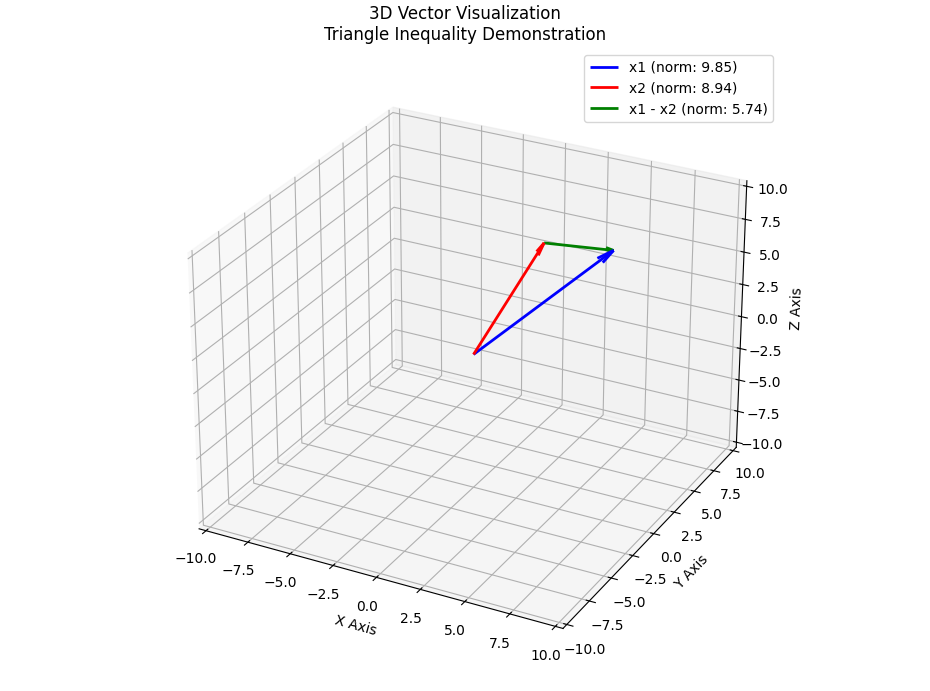
\includegraphics[width=0.9\textwidth,height=0.7\textheight,keepaspectratio]{figurer/Inv_Triangle_ineq.png}
\end{center}


Merk at for en generell norm, så er 
\begin{align*}
    \left\lVert u - v \right\rVert &= \left\lVert \left( -1 \right) \left( v - u \right) \right\rVert \\
    &= \left| -1 \right| \left\lVert v-u \right\rVert \\
    &= \left\lVert v-u \right\rVert 
\end{align*}


\section*{3.2 Konvergens}
\addcontentsline{toc}{section}{Konvergens}

\begin{definitionbox}{3.2.1}{}
En følge av vektorer i et vektorrom U er en uendelig lang liste $ \left( u_1, u_2, ... \right)  $ hvor $ u_1, u_2, ... \in  U $ 
\end{definitionbox}

\begin{definitionbox}{3.2.2}{}
La  være et normert vektorrom. La $ \left( u_k \right) _{k \in \mathbb{N}} $ være en følge av vektorer, og la $ u \in U $. Vi sier at \textbf{\textit{følgen konvergerer mot u }} og skriver $ u_k \to u $ eller $ \lim_{k \to \infty} u_k = u $, dersom det for enhver $ \eps > 0 $ finnes en $ n \in \mathbb{N} $ slik at 
\[
    k \geq n \rightarrow \left\lVert u_k - u \right\rVert < \eps
\]
\end{definitionbox}

\begin{oppgavebox}{3.2.3}{}
Forklar hvorfor følgende er ekvivalent
\begin{itemize}
    \item Følgen av vektorer $ \left( u_k \right) _{k \in \mathbb{N}} $ konvergerer mot u
    \item Følgen av reelle tall $ \left( \left\lVert u_k - u \right\rVert  \right)_{k \in \mathbb{N}}  $ konvergerer mot 0
\end{itemize}

\begin{proofbox}{3.2.3}{}
Anta først at følgen $ \left( u_k \right) _{k \in \mathbb{N}} $ konvergerer mot 0. Det vil si at for en $ k\geq N $ hvor $ N \in \mathbb{N} $, så er $ \left\lVert u_k - u \right\rVert < \eps $, gitt en $ eps > 0 $ . Det vil si at den uendelige følgen $ \left( \left\lVert u_k - u \right\rVert \right)_{k \in \mathbb{N}}  $ konvergerer mot 0\\

Anta motsatt at følgen $ \left( \left\lVert u_k - u \right\rVert  \right)_{k \in \mathbb{N}}  $ konvergerer mot 0.Gitt en $ eps > 0 $, finnes da en $ N \in \mathbb{N} $ som er slik at for alle $ k \geq N $, er $ \left\lVert u_k - u \right\rVert < \eps $\\

Vi konkluderer med at begge påstandene er ekvivalente
\end{proofbox}
\end{oppgavebox}

\begin{oppgavebox}{3.2.4}{}
Vi betrakter vektorrommet $ \ell^2 (\mathbb{R}) $ med normen $ \left\lVert \cdot \right\rVert _{\ell^1} $. La $ u_1, ..., u_n \in \ell^2 (\mathbb{R}) $ være vektorene
\[
    u_k := \left( 1, \frac{ 1 }{ 2 }, \frac{ 1 }{ 4 }, ..., \frac{ 1 }{ 2^k } \right) \; \forall k \in \mathbb{N}
\]
Konvergerer følgen $ \left( u_k \right) _{k \in \mathbb{N}} $? Hva er isåfall grensen? 
\end{oppgavebox}


\begin{definitionbox}{3.2.5}{}
La U være et normert vektorrom $ u \in U $ og $ r > 0 $. \textbf{\textit{Den åpne kula sentrert i u med radius r}} er mengden
\[
    B_r(u) := \left\{ v \in U : \left\lVert u - v \right\rVert < r \right\} 
\]\\

\textbf{\textit{Den lukkede kula sentrert i u med radius r}} er definert som
\[
    \overline{B_r}(u) := \left\{ v \in U : \left\lVert u - v \right\rVert \leq r \right\} 
\]
\end{definitionbox}

\begin{definitionbox}{3.2.6}{}
La U vøre et normert vektorrom, og la $E \subseteq U $ være en delmengde
\begin{itemize}
    \item E er \textbf{\textit{åpen}} om for enhvert $ u \in E \; \exists $ en $ \delta > 0 $ s.a. $ B_{\delta} (u) \subseteq E $. Med andre ord er E åpen hvis det for enhver $ u \in E $ finnes en $ \delta > 0 $ slik at for enhver $ v \in U $ med $ \left\lVert u - v \right\rVert < \delta  $, så er også $ v \in  E $
    \item E er \textbf{\textit{lukket}} om det for enhver konvergent følge $ \left( u_k \right) _{k \in \mathbb{N}} $ av vektorer $ u_k \in E $  er slik at også $ \lim_{k \to \infty} u_k \in E $
    \item E er \textbf{\textit{begrenset}} om $ \exists  \; r > 0$  s.a. $ E \subseteq B_r(0) $ 
\end{itemize}
\end{definitionbox}

\begin{oppgavebox}{3.2.7}{}
Vis at
\begin{itemize}
    \item alle kuler er begrensede
    \item alle åpne kuler $ B_r(u) $ er åpne mengder
    \item alle lukkene kuler $ \overline{B_r}(u) $ er lukkede mengder
\end{itemize}

Hint: I ii) lar du $ v \in B_r(u) $ og må finne en $ s>0 $ s.a. $ B_s(v)  \subseteq B_r(u)$. I alle tre bruk trekantulikheten

\begin{proofbox}{3.2.7 a)}{}
Jeg viser for alle lukkede kuler. Svaret gjelder da uansett for åpne kuler. La $ \overline{B_r}(u)  $ være en lukket kule. Definer Så
\[
    R := r + \left\lVert u \right\rVert + 1
\]
Da er $ \forall v \in U $ $ \left\lVert v - 0 \right\rVert = \left\lVert \left( v-u \right) +u  \right\rVert \leq \left\lVert v-u \right\rVert + \left\lVert u \right\rVert   $ 

Siden $ \overline{B_r}(u)  $ er kule som er hele området om u slik at $ \left\lVert u - v \right\rVert \leq r $ , og vi har definert $ R $ som $ r + \left\lVert u \right\rVert +1 $, så vet vi da at 

\[
    \left\lVert v \right\rVert \leq \left\lVert v - u \right\rVert + \left\lVert u \right\rVert \leq r + \left\lVert u \right\rVert < R = r + \left\lVert u \right\rVert + 1
\] 
\end{proofbox}

\begin{proofbox}{3.2.7 b)}{}
La $ v \in  B_r(u) $ og definer $ s := r - \left\lVert u - v \right\rVert  $. La så en $ w \in B_s(v) $. Da er 
\[
    \left\lVert u - w \right\rVert \leq \left\lVert u - v \right\rVert + \left\lVert v - w \right\rVert \leq \left\lVert u - v \right\rVert + s = \left\lVert u - v \right\rVert + r - \left\lVert u-v \right\rVert = r
\]
Dermed har jeg vist at $ w \in B_r(u) $ i tillegg til $ B_s(v) $, altså $ B_s(v) \subseteq B_r(u) $. Dette utsagnet er nå sant fordi $ s < r $ 
\end{proofbox}

\begin{proofbox}{3.2.7 c)}{}
La $ \left( v_k \right) _{k \in \mathbb{N}} $ være en følge i $ \overline{B_r}(u) $ . Da er 
\[
    \left\lVert u - v \right\rVert \leq \left\lVert u - v_k \right\rVert + \left\lVert v_k - v \right\rVert \leq r + \left\lVert v_k - v \right\rVert 
\]
Siden $ v_k \to v $ når $ k \to \infty $, så er $ \left\lVert u - v \right\rVert \leq r $. Derfor er alle lukkede kuler en lukket mengde.
\end{proofbox}
\end{oppgavebox}

\begin{oppgavebox}{3.2.8}{}
La U være et normert vektorrom. Vis at U
\begin{itemize}
    \item Er en åpen delemngde av U
    \item er en lukket delemengde av U
    \item er bregrenset kun hvis $ U = \left\{ 0 \right\}  $ 
\end{itemize}

\begin{proofbox}{3.2.8 a)}{}

\end{proofbox}
\end{oppgavebox}


\section*{3.3 Kontinuitet}
\addcontentsline{toc}{section}{Kontinuitet}

\begin{definitionbox}{3.3.1}{}
La U og V være normerte vektrorrom, og la $ E \subseteq U $. Vi sier at en funksjon $ f: E \to V $  er \textbf{\textit{kontinurlig i et punkt $ u \in E $ }} om det for enhver $ \eps > 0 $ finnes en $ \delta > 0 $ s.a.
\[
    v \in U, \left\lVert u - v \right\rVert_U < \delta \rightarrow \left\lVert f(u) - f(v) \right\rVert _V < \eps
\]
f er kontinuerlig overalt hvis f er kontinuerlig i alle punkter $ u \in E $. Mengden med alle kontinuerlige funksjoner fra E til V kalles for $ C^0 \left( E, V \right)  $ 
\end{definitionbox}

\begin{oppgavebox}{3.3.2}{}
$ f: E \to V $ er Lipschitz kontinuerlig hvis $ \exists L > 0 $ s.a.
\[
    \left\lVert f(u) - f(v) \right\rVert _V \leq L \left\lVert u - v \right\rVert _U \; \forall u, v \in E
\]
Vis at alle Lipschitz kontinuerlige funksjoner er kontinuerlige.
\begin{proofbox}{3.3.2}{}
Anta at $ f: E \to V $ er Lipschitz kont. Da $ \exists L >0 $ s.a.
\[
    \left\lVert f(u) - f(v) \right\rVert _V \leq L \left\lVert u - v \right\rVert _E
\]
Plukk $ \delta = \frac{ \epsilon   }{ L } $. For enhver $ u \in E $ som oppfyller $ \left\lVert u - v \right\rVert _E $ har vi at $ \left\lVert f(u) - f(v) \right\rVert _V \leq L \left\lVert u - v \right\rVert _E < L \frac{ \epsilon }{ L } = \epsilon  $. Dette viser at for en $ \epsilon > 0 $ finnes det en $ \delta > 0 $ slik at $ \left\lVert u - v \right\rVert _E \delta \rightarrow \left\lVert f(u) - f(v) \right\rVert _V < \epsilon  $. Altså er f kontinuerlig i u, fordi u var vilkårlig
\end{proofbox}
\end{oppgavebox}

\begin{propositionbox}{3.3.3}{}
La U, V, E og f være som i 3.3.1. Da er f kontinuerlig i $ u E $ om følgende gjelder:\\

Om $ \left( u_k \right) _{k \in \mathbb{N}} $ er en følge i E som konvergerer mot u i E, så konvergerer følgen $ \left( f(u_k) \right) _{k \in  \mathbb{N}} \to f(u)$ 
\begin{proofbox}{3.3.3}{}
    Se boken
\end{proofbox}
\end{propositionbox}

\begin{oppgavebox}{3.3.4}{}
Bevis følgende

\begin{itemize}
    \item Om $ f : U \to V  $ og $ g: V \to W $ er kont, er også $ g \circ f  $ kont
    \item $ f:U \to \mathbb{R} $ gitt ved $ f(u) := \left\lVert u \right\rVert _U $ er kont
    \item Om $ f: U \to V $ er kont og $ F \subseteq V $ er åpen, er også 
    \[
        f^{-1}(F) := \left\{ u \in U : f(u) \in F \right\} 
    \]
    åpen
    \item Om $ f: U \to V $ er kont og $ F \subseteq V $ er lukket, er også $ f^{-1}(F)  $  lukket
    
\end{itemize}

\begin{proofbox}{3.3.4 a)}{}
om $ f: U \to V $ er kont, er det en følge $ \left( f(u_k) \right) _{k \in \mathbb{N}} $ som er konvergent. Av 3.3.3, er da også $ \left( g \left( f \left( u_k \right)  \right)  \right)_{k \in \mathbb{N}}  $ også konvergent, og dermed av samme 3.3.3, er da $ g\circ f: U \to W $ kontinuerlig
\end{proofbox}

\begin{proofbox}{3.3.4 b)}{}

\end{proofbox}
\end{oppgavebox}

\end{document}